\documentclass[14pt]{extbook}
\usepackage{multicol, enumerate, enumitem, hyperref, color, soul, setspace, parskip, fancyhdr} %General Packages
\usepackage{amssymb, amsthm, amsmath, bbm, latexsym, units, mathtools} %Math Packages
\everymath{\displaystyle} %All math in Display Style
% Packages with additional options
\usepackage[headsep=0.5cm,headheight=12pt, left=1 in,right= 1 in,top= 1 in,bottom= 1 in]{geometry}
\usepackage[usenames,dvipsnames]{xcolor}
\usepackage{dashrule}  % Package to use the command below to create lines between items
\newcommand{\litem}[1]{\item#1\hspace*{-1cm}\rule{\textwidth}{0.4pt}}
\pagestyle{fancy}
\lhead{Progress Quiz 9}
\chead{}
\rhead{Version C}
\lfoot{8590-6105}
\cfoot{}
\rfoot{Fall 2020}
\begin{document}

\begin{enumerate}
\litem{
Solve the quadratic equation below. Then, choose the intervals that the solutions $x_1$ and $x_2$ belong to, with $x_1 \leq x_2$.\[ 20x^{2} +69 x + 54 = 0 \]\begin{enumerate}[label=\Alph*.]
\item \( x_1 \in [-4.55, -4.41] \text{ and } x_2 \in [-0.72, -0.6] \)
\item \( x_1 \in [-45.28, -44.69] \text{ and } x_2 \in [-24.1, -23.91] \)
\item \( x_1 \in [-2.84, -1.36] \text{ and } x_2 \in [-1.21, -1.17] \)
\item \( x_1 \in [-9.86, -8.53] \text{ and } x_2 \in [-0.34, -0.11] \)
\item \( x_1 \in [-3.95, -3.52] \text{ and } x_2 \in [-0.81, -0.68] \)

\end{enumerate} }
\litem{
Write the equation of the graph presented below in the form $f(x)=ax^2+bx+c$, assuming  $a=1$ or $a=-1$. Then, choose the intervals that $a, b,$ and $c$ belong to.
\begin{center}
    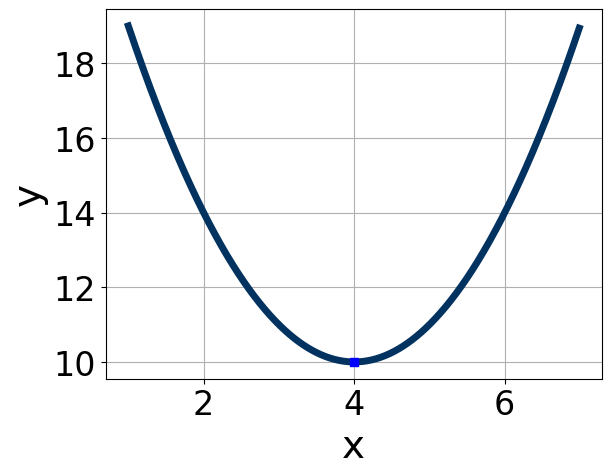
\includegraphics[width=0.5\textwidth]{../Figures/quadraticGraphToEquationC.png}
\end{center}
\begin{enumerate}[label=\Alph*.]
\item \( a \in [0, 2], \hspace*{5mm} b \in [-9, -7], \text{ and } \hspace*{5mm} c \in [6, 9] \)
\item \( a \in [-5, 0], \hspace*{5mm} b \in [-9, -7], \text{ and } \hspace*{5mm} c \in [-28, -22] \)
\item \( a \in [0, 2], \hspace*{5mm} b \in [6, 12], \text{ and } \hspace*{5mm} c \in [6, 9] \)
\item \( a \in [-5, 0], \hspace*{5mm} b \in [6, 12], \text{ and } \hspace*{5mm} c \in [-28, -22] \)
\item \( a \in [0, 2], \hspace*{5mm} b \in [6, 12], \text{ and } \hspace*{5mm} c \in [24, 27] \)

\end{enumerate} }
\litem{
Solve the quadratic equation below. Then, choose the intervals that the solutions belong to, with $x_1 \leq x_2$ (if they exist).\[ 20x^{2} -12 x -9 = 0 \]\begin{enumerate}[label=\Alph*.]
\item \( x_1 \in [-29.65, -28.46] \text{ and } x_2 \in [29.54, 30.7] \)
\item \( x_1 \in [-0.6, -0.14] \text{ and } x_2 \in [0.44, 1.97] \)
\item \( x_1 \in [-9.31, -8.17] \text{ and } x_2 \in [20.25, 21.48] \)
\item \( x_1 \in [-1.33, -0.95] \text{ and } x_2 \in [0.38, 0.91] \)
\item \( \text{There are no Real solutions.} \)

\end{enumerate} }
\litem{
Write the equation of the graph presented below in the form $f(x)=ax^2+bx+c$, assuming  $a=1$ or $a=-1$. Then, choose the intervals that $a, b,$ and $c$ belong to.
\begin{center}
    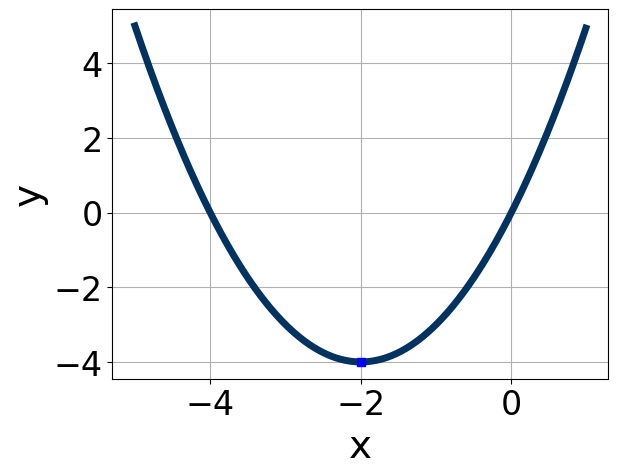
\includegraphics[width=0.5\textwidth]{../Figures/quadraticGraphToEquationCopyC.png}
\end{center}
\begin{enumerate}[label=\Alph*.]
\item \( a \in [-1, 0], \hspace*{5mm} b \in [1, 9], \text{ and } \hspace*{5mm} c \in [3, 7] \)
\item \( a \in [0, 3], \hspace*{5mm} b \in [-7, -1], \text{ and } \hspace*{5mm} c \in [12, 17] \)
\item \( a \in [0, 3], \hspace*{5mm} b \in [1, 9], \text{ and } \hspace*{5mm} c \in [12, 17] \)
\item \( a \in [0, 3], \hspace*{5mm} b \in [-7, -1], \text{ and } \hspace*{5mm} c \in [-6, -2] \)
\item \( a \in [-1, 0], \hspace*{5mm} b \in [-7, -1], \text{ and } \hspace*{5mm} c \in [3, 7] \)

\end{enumerate} }
\litem{
Solve the quadratic equation below. Then, choose the intervals that the solutions belong to, with $x_1 \leq x_2$ (if they exist).\[ -12x^{2} -7 x + 3 = 0 \]\begin{enumerate}[label=\Alph*.]
\item \( x_1 \in [-0.53, -0.26] \text{ and } x_2 \in [0.67, 1.29] \)
\item \( x_1 \in [-15.04, -14.04] \text{ and } x_2 \in [12.58, 14.45] \)
\item \( x_1 \in [-3.9, -3.28] \text{ and } x_2 \in [10.4, 11.5] \)
\item \( x_1 \in [-1.84, -0.6] \text{ and } x_2 \in [-0.37, 0.86] \)
\item \( \text{There are no Real solutions.} \)

\end{enumerate} }
\litem{
Graph the equation below.\[ f(x) = -(x+1)^2 - 15 \]\begin{enumerate}[label=\Alph*.]
\begin{multicols}{2}\item 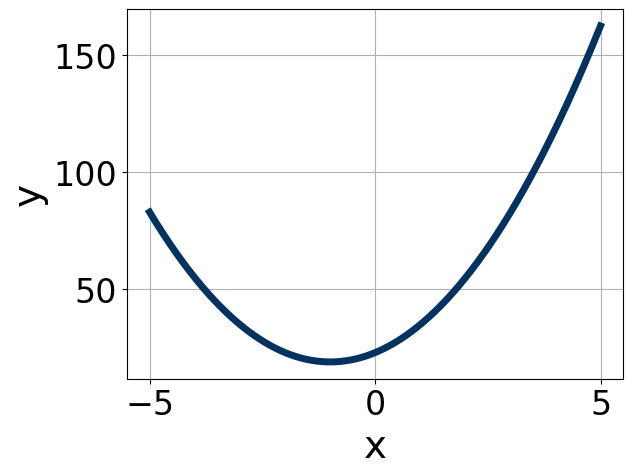
\includegraphics[width = 0.3\textwidth]{../Figures/quadraticEquationToGraphCopyAC.png}\item 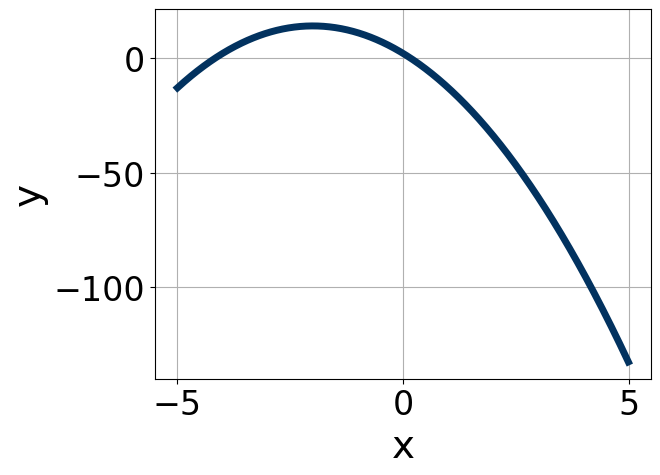
\includegraphics[width = 0.3\textwidth]{../Figures/quadraticEquationToGraphCopyBC.png}\item 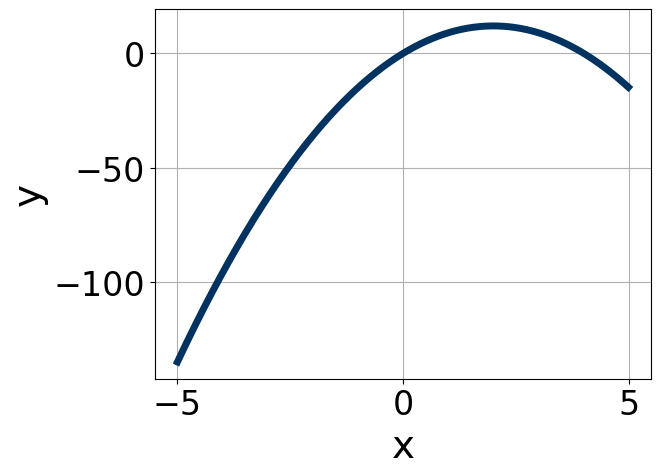
\includegraphics[width = 0.3\textwidth]{../Figures/quadraticEquationToGraphCopyCC.png}\item 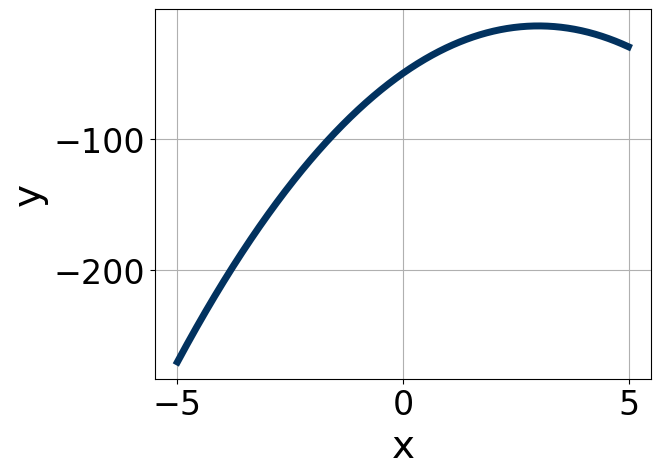
\includegraphics[width = 0.3\textwidth]{../Figures/quadraticEquationToGraphCopyDC.png}\end{multicols}\item None of the above.
\end{enumerate} }
\litem{
Solve the quadratic equation below. Then, choose the intervals that the solutions $x_1$ and $x_2$ belong to, with $x_1 \leq x_2$.\[ 15x^{2} +2 x -24 = 0 \]\begin{enumerate}[label=\Alph*.]
\item \( x_1 \in [-20.32, -19.63] \text{ and } x_2 \in [17.74, 19.67] \)
\item \( x_1 \in [-1.79, -1.02] \text{ and } x_2 \in [1.02, 1.57] \)
\item \( x_1 \in [-4.01, -3.93] \text{ and } x_2 \in [-0.24, 0.53] \)
\item \( x_1 \in [-2.95, -2.34] \text{ and } x_2 \in [0.5, 0.82] \)
\item \( x_1 \in [-0.95, -0.22] \text{ and } x_2 \in [3.3, 4.35] \)

\end{enumerate} }
\litem{
Factor the quadratic below. Then, choose the intervals that contain the constants in the form $(ax+b)(cx+d); b \leq d.$\[ 24x^{2} +50 x + 25 \]\begin{enumerate}[label=\Alph*.]
\item \( a \in [10.31, 12.56], \hspace*{5mm} b \in [4, 10], \hspace*{5mm} c \in [1.67, 3.04], \text{ and } \hspace*{5mm} d \in [5, 7] \)
\item \( a \in [0.28, 1.33], \hspace*{5mm} b \in [12, 24], \hspace*{5mm} c \in [-0.29, 1.88], \text{ and } \hspace*{5mm} d \in [29, 32] \)
\item \( a \in [1.11, 3.63], \hspace*{5mm} b \in [4, 10], \hspace*{5mm} c \in [10.61, 12.95], \text{ and } \hspace*{5mm} d \in [5, 7] \)
\item \( a \in [2.98, 4.99], \hspace*{5mm} b \in [4, 10], \hspace*{5mm} c \in [5.81, 7.5], \text{ and } \hspace*{5mm} d \in [5, 7] \)
\item \( \text{None of the above.} \)

\end{enumerate} }
\litem{
Factor the quadratic below. Then, choose the intervals that contain the constants in the form $(ax+b)(cx+d); b \leq d.$\[ 36x^{2} -60 x + 25 \]\begin{enumerate}[label=\Alph*.]
\item \( a \in [2.4, 4.7], \hspace*{5mm} b \in [-8, -2], \hspace*{5mm} c \in [10.18, 13.1], \text{ and } \hspace*{5mm} d \in [-8, -4] \)
\item \( a \in [16.3, 18.1], \hspace*{5mm} b \in [-8, -2], \hspace*{5mm} c \in [1.76, 2.44], \text{ and } \hspace*{5mm} d \in [-8, -4] \)
\item \( a \in [-1.6, 1.7], \hspace*{5mm} b \in [-30, -21], \hspace*{5mm} c \in [0.16, 1.82], \text{ and } \hspace*{5mm} d \in [-30, -27] \)
\item \( a \in [4.6, 9.6], \hspace*{5mm} b \in [-8, -2], \hspace*{5mm} c \in [4.79, 6.93], \text{ and } \hspace*{5mm} d \in [-8, -4] \)
\item \( \text{None of the above.} \)

\end{enumerate} }
\litem{
Graph the equation below.\[ f(x) = (x+2)^2 - 13 \]\begin{enumerate}[label=\Alph*.]
\begin{multicols}{2}\item 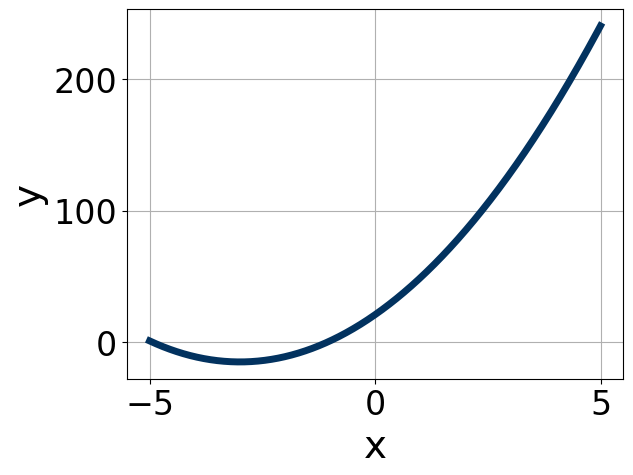
\includegraphics[width = 0.3\textwidth]{../Figures/quadraticEquationToGraphAC.png}\item 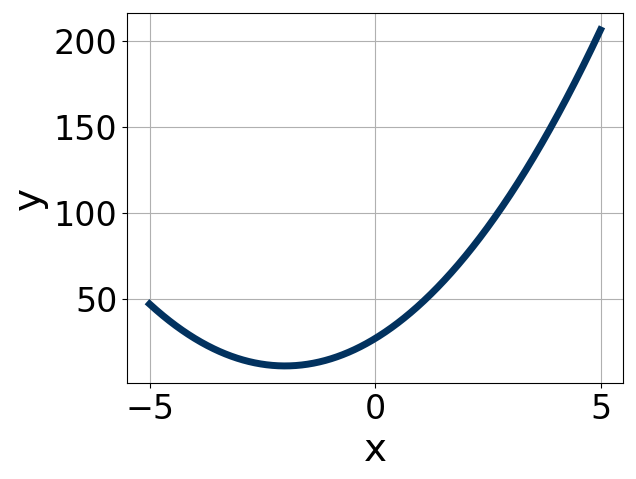
\includegraphics[width = 0.3\textwidth]{../Figures/quadraticEquationToGraphBC.png}\item 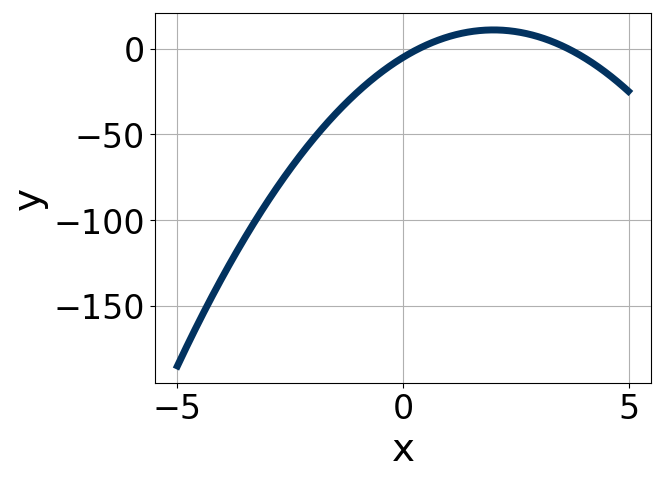
\includegraphics[width = 0.3\textwidth]{../Figures/quadraticEquationToGraphCC.png}\item 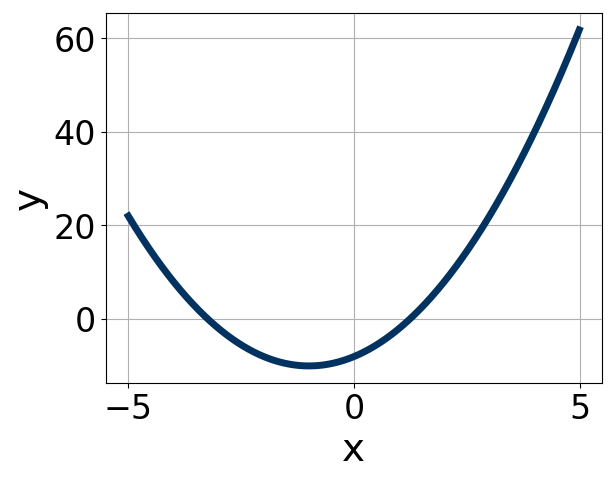
\includegraphics[width = 0.3\textwidth]{../Figures/quadraticEquationToGraphDC.png}\end{multicols}\item None of the above.
\end{enumerate} }
\end{enumerate}

\end{document}